\chapter{Discussion}

The results show that optimizing a path to achieve better observation of the ground path while using a fixed camera is a difficult optimization problem to solve. However, the results also show that tracking can be improved by following an optimized path.

\section{Piecewise Linear Vs. Curved Paths}

There was a big difference in how well the MPC handles piecewise linear and curved paths. While it managed to optimize curved turns as sharp as $90\degree$ with a $50$m radius, it couldn't optimize linear corners sharper than $45\degree$.

The difference in how well it performs is most likely due to the fact that the piecewise linear paths consists of actual corners, which do not give the same smooth change in reference that curved paths do. These linear corners do not represent a path that a fixed-wing UAV would naturally travel. However, since no processing is performed on the path before it is used as a reference to the optimization problem, the optimization algorithm will try to find a solution that do follow these corners. If some more processing was put into the trajectory generation, it would have been possible to smooth out the corners before they were fed to the optimization algorithm, making it more similar to a curved path.

As shown in the results, the MPC is able to optimize a $70\degree$ linear corner when the stepsize is reduced from $0.2$s to $0.1$s. This makes sense with the rapid changing reference, since the MPC is able to respond to rapid changes in reference quicker with a shorter stepsize. However, the application is very time consuming even when using a stepsize of $0.2$s, and decreasing the stepsize would increase this duration, as both the number of intervals and number of steps in the horizon would need to be increased to achieve good results.

A more surprising result when comparing piecewise linear and curved paths is that the linear paths gave a more precise result during simulation. As was seen when comparing the optimization result for curved and linear paths, the linear paths required sharper changes in the roll angle. This information is not embedded in the optimized path, and thus it was not expected that tracking the optimized path would give a better result in the linear case.


\section{Generating a Precise Trajectory}

For some of the results in this thesis it is suspected that a particular set of unfortunate waypoints can cause instability. The reason for this suspicion is the way the trajectory is generated for every iteration of the MPC, described in section \ref{subseq:generating_trajectory}. This method assumes that the UAV will maintain a constant speed, in order to calculate the distance the UAV will travel during one timestep. This assumption will introduce some inaccuracies, but the results show that during stable optimizations the speed did not vary much. However, this method of generating the trajectory introduces another inaccuracy, related to the parametrization of the path.

A parametrized path consists of several points spaced by a given distance. For this reason, when processing the reference path, it is not always possible to find a point that is exactly the desired distance away from the UAV. To avoid this, points with a distance away that is within a given range is accepted as the next waypoint. If this range is too big the inaccuracy will be too big, which will cause a spike in the reference model in the cost function. Because of this spike in reference the optimization algorithm will seek to follow the spike, which causes the oscillations in the states.

\begin{figure}[]
	\centering
    \makebox[\textwidth][c]{
	\subfloat[Roll angle]{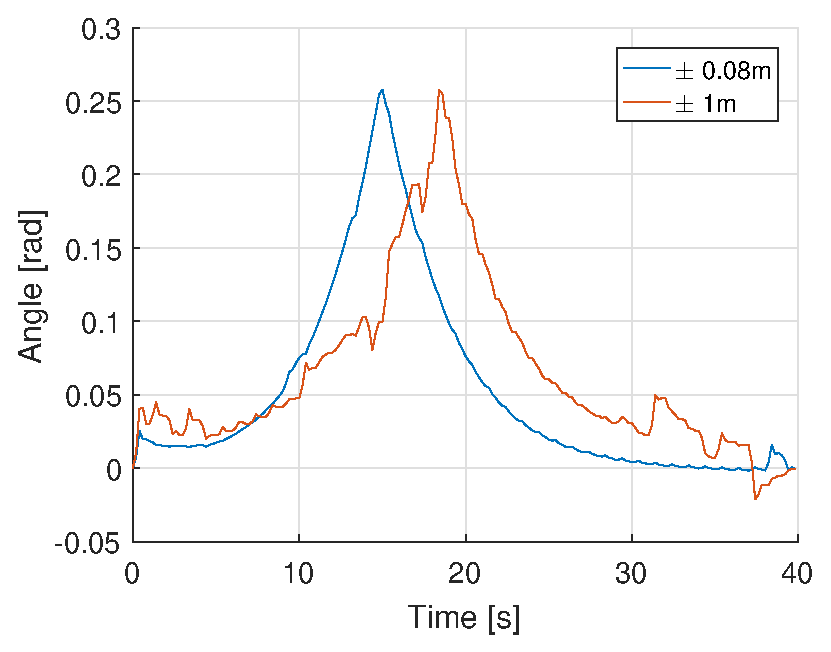
\includegraphics[width=0.5\textwidth, keepaspectratio=true]{../../results/opt/turns/linear/fig_45deg/roll_comparison.eps}
	\label{fig:bad_roll}}
	\qquad
	\subfloat[Camera Position for $\pm 1$m]{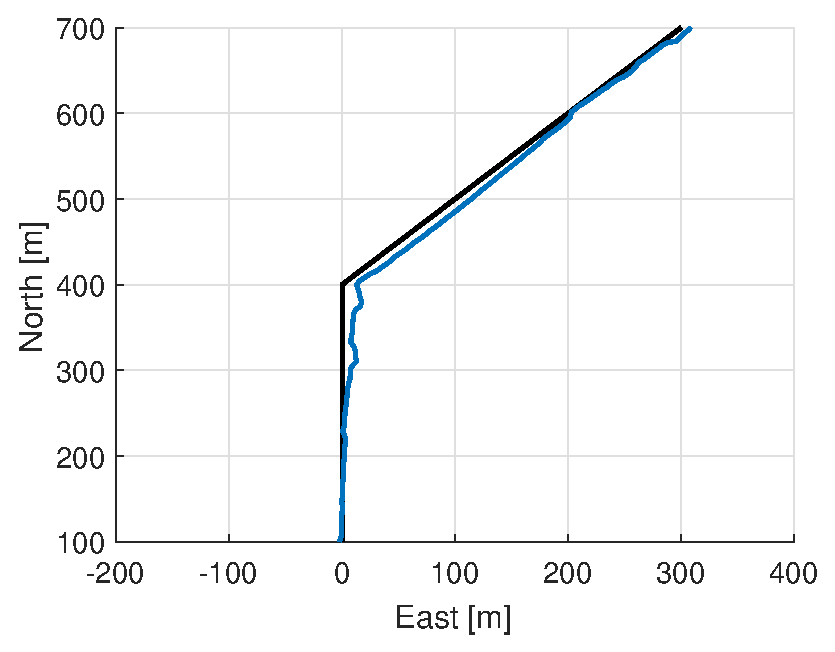
\includegraphics[width=0.5\textwidth, keepaspectratio=true]{../../results/opt/turns/linear/fig_45deg/bad_cam.eps}
	\label{fig:bad_cam}}}
	\caption{The effect of difference acceptance rates for waypoints.}
	\label{fig:oscillating_attitude}
\end{figure}

In Figure \ref{fig:oscillating_attitude} the effect the acceptance range of waypoints has on the roll through a $45\degree$ linear turn is shown. First of all, the tracking of the ground path was worse, as can be seen in Figure \ref{fig:bad_cam}. And as can be seen in Figure \ref{fig:bad_roll}, the roll angle contains more oscillations when the acceptance rate is $\pm 1$m, compared to $\pm 0.08$m. While this is as expected, it proves that the precision is important when generating the trajectory.

\section{Cost Function}

The cost function in this thesis consisted of eight states, where the position of the camera were the states included to solve the problem of finding an optimal path to track with a fixed camera. While this cost function do solve the problem, it does have some problems related to the tuning of it.

Early in testing, before the final tuning of the cost function had been decided, it was clear that the easiest way to solve the control problem was to control the course of the airplane using the rudder. This is an easy solution to the problem since it does not rely on using the roll angle that inherently shifts the camera position. Since this thesis aimed to create an optimal path that could be used with a bank-to-turn controller, this behaviour had to be removed. This was done be heavily punishing usage of rudder, while there was almost no weight put on the usage of ailerons.

Weighting the usage of rudder more than aileron worked as intended: The MPC uses roll to follow the path instead of yaw. However, the light weighting of aileron input caused it to oscillate heavily, adding to the effect of the poor trajectory generation previously mentioned.

Another problem discovered during testing was how the MPC deals with long stretches of path. When the turns were positioned closely after one another it was no problem, as the MPC would have to change the course of the aircraft often. When optimizing the lawnmover path in section \ref{subsec:lawnmover} however, it became clear that the MPC chose to position the camera centre point on the ground path by keeping a constant roll angle and flying next to the path. Since the cost function only seeks to minimize the control rates, this was a cheap solution that required no change of the control states.

One possible solution to this would be to include the position of the UAV in the cost function. These terms would have to be weighted lower than the position of the camera since the camera position is the main focus, but it would cause flying next to the path a more expensive solution compared to flying just above the path. Another solution may be to include control surface deflection in the cost function, but this is most likely a bad decision as some situations require a constant deflection of the control surfaces.


\section{Control Signals}

\begin{figure}[]
	\centering
    \makebox[\textwidth][c]{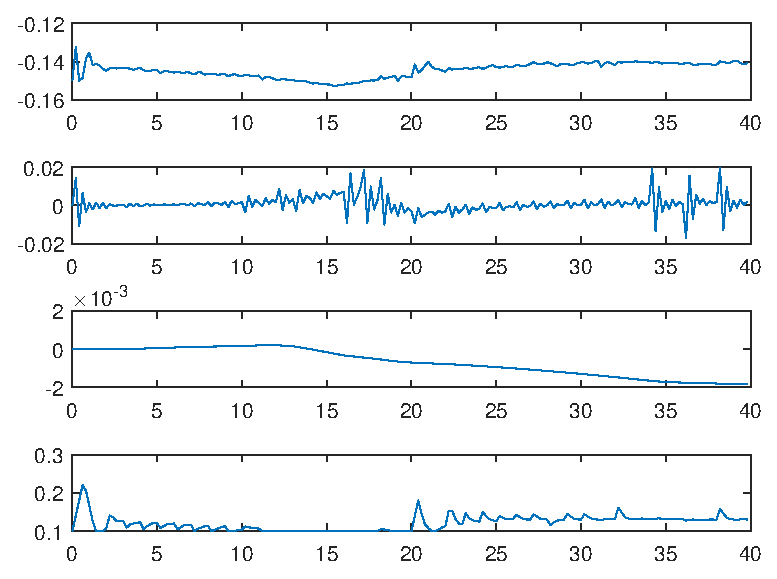
\includegraphics[width=0.8\textwidth, keepaspectratio=true]{../../results/opt/turns/curved/fig_45deg/control.eps}}
	\caption{The control signals when optimizing a $45\degree$ curved turn.}
	\label{fig:control_signals}
\end{figure}

In this report no plots of the control signals have been given. The main reason for this is that the output of the MPC is the optimized path, and the control signals are not intended to be used for tracking the path. Another reason can be seen in Figure \ref{fig:control_signals}: they do not always make sense. There are two reasons for this.

First of all, the noise is most likely related to the oscillations previously mentioned in this chapter. For every iteration of the MPC there is a significant spike in all of the four control signals, some more than others. Since there is a spike in the reference for every iteration, it is no surprise there is a spike in the control signals with that spike.

The second reason is that the control signals for the aileron and rudder are surprisingly small, and the aileron control signal often do not match the roll angle of the aircraft. The reason for this is most likely tied to the linearized model. The model is already an approximation of the real model, and poor selection of parameters may make matters worse.

Since the UAV states seem reasonable, it was decided not to give much weight to the control signals in this thesis. %However, the results show that there might be precision to gain from using angle rates or control signals to optimize output, and for this usage more precise control signals are needed.